% This is a sample document using the University of Minnesota, Morris, Computer Science
% Senior Seminar modification of the ACM sig-alternate style. Much of this content is taken
% directly from the ACM sample document illustrating the use of the sig-alternate class. Certain
% parts that we never use have been removed to simplify the example, and a few additional
% components have been added.

% See https://github.com/UMM-CSci/Senior_seminar_templates for more info and to make
% suggestions and corrections.

\documentclass{sig-alternate}
\usepackage{color}
\usepackage{graphicx}
\usepackage{mathtools}
\usepackage{array}
%\usepackage[colorinlistoftodos]{todonotes}

%%%%% Uncomment the following line and comment out the previous one
%%%%% to remove all comments
%%%%%\newcommand{\comment}[1]{}
\newcommand{\comment}[1]{{\bf \tt  {#1}}}
%%%%% NOTE: comments still occupy a line even if invisible;
%%%%% Don't write them as a separate paragraph
\newcommand{\todo}[1]{\textcolor{magenta}{\comment{Todo: {#1}}}}

\begin{document}

% --- Author Metadata here ---
%%% REMEMBER TO CHANGE THE SEMESTER AND YEAR
\conferenceinfo{UMM CSci Senior Seminar Conference, May 2015}{Morris, MN}

\title{Monte Carlo Tree Search and Its Applications}

\numberofauthors{1}

\author{
% The command \alignauthor (no curly braces needed) should
% precede each author name, affiliation/snail-mail address and
% e-mail address. Additionally, tag each line of
% affiliation/address with \affaddr, and tag the
% e-mail address with \email.
\alignauthor
Max Magnuson\\
	\affaddr{Division of Science and Mathematics}\\
	\affaddr{University of Minnesota, Morris}\\
	\affaddr{Morris, Minnesota, USA 56267}\\
	\email{magnu401@morris.umn.edu}
}

\maketitle
\begin{abstract}
Monte Carlo tree search (MCTS) is a probabilistic algorithm that uses lightweight random simulations to selectively grow a game tree. MCTS has experienced a lot of success in domains with large search spaces which historically have challenged deterministic algorithms~\cite{RAVEinGo}. This paper discusses the steps of the MCTS algorithm, its application to the board game Go, and its application to narrative generation. 
\end{abstract}

\keywords{Monte Carlo Tree Search, Heuristics, Upper Confidence Bounds, Artificial Intelligence}

\section{Introduction} 
In 1997 the field of artificial intelligence(AI) experienced a monumental breakthrough when IBM's Deep Blue defeated Garry Kasparov, a reigning grand master, in a chess match~\cite{TheGrandChallenge}. The researchers achieved this by using brute force deterministic tree searching methods combined with human knowledge of chess. The human knowledge allows the AI to evaluate the strategic value of a move much like a grand master would, and then populate a tree to search for the best move. This event demonstrated to the world the power of computers and artificial intelligence. 

While computers are capable of outplaying the top players of chess, the deterministic strategies that they employ do not scale well into larger search spaces. When there are too many options available, the deterministic nature of these algorithms take too long evaluating every option and quickly are overwhelmed. Two applications with very large search spaces are Go which is a board game about positional advantage and narrative generation. Go has many more moves available to the player than in chess, and each of those moves can have major effects on moves 50 to 100 moves ahead~\cite{RAVEinGo}. This makes the game trees in Go much wider and deeper which vastly increases the complexity. 

Narrative generation has some of the same problems. As the number of characters, items, locations, and actions increase, the search space grows tremendously. An algorithm needs access to plenty of these agents to produce interesting narratives, but there are just too many possible interactions for deterministic algorithms.

In order to address problems with large search spaces, we must turn to alternative methods. One such method, Monte Carlo tree search (MCTS), has had a lot of success in Go and in other applications~\cite{TheGrandChallenge}~\cite{ActionSelection}. MCTS eschews the typical brute force tree searching methods, and utilizes statistical processes instead. This makes MCTS a probabilistic algorithm. As such, it will not always choose the best action, but it still performs reasonably well given sufficient time and memory. MCTS performs lightweight simulations which randomly selects actions. These simulations are used to selectively grow a tree over a large number of iterations. Since these simulations do not take long to perform, it allows MCTS to explore search spaces quickly. This is what gives MCTS the advantage over deterministic methods in large search spaces.

With MCTS capable of surmounting problems with large search spaces, AI can now perform well in new areas. In 2009, for the first time ever, a computer defeated a top professional Go player in a 9x9 game~\cite{TheGrandChallenge}. It took twelve years for AI to advance from defeating Garry Kasparov to achieve its first major victory in Go, and it was only on the smallest board that Go is played on. While not as publicized as deep blue's victory, it displays the power of MCTS.

MCTS has been growing in popularity in recent years, and it demonstrates a lot of promise. In this paper, we will examine the naive implementation of MCTS, its applications to Go, and its applications to narrative generation.  
\section{Background}
MCTS combines the random sampling of traditional Monte Carlo methods with tree searching. Monte Carlo methods use repeated random sampling to obtain results. In MCTS, the random sampling is in the form of random simulations which are used to expand the game tree. MCTS is an iterative algorithm that traverses and expands the tree on each iteration. The tree traversal uses statistical processes, and the MCTS algorithm relies on the convergence of the traversal to reliably choose the best move. The traversal is in convergence when the same path is selected during each iteration. MCTS is a probabilistic method that does not always find the optimal move, but it has reasonably high success at choosing moves that will lead to greater chances of winning.
\subsection{The Tree Structure}\label{sec:TreeStructure}


MCTS encodes the game state and its potential moves into a tree. Each node in the tree represents a potential game state with the root node representing the current state. Each edge represents a legal move that can be made from one game state to another. In other words, it represents the transformation from the parent node to the child node. Any node may have as many children as there are legal moves. For example, at the start of a game of TicTacToe the root node may have up to nine children, one for each possible move. Each following child can only have one less child than its parent since the previous moves are no longer available as options.

\begin{figure}[h]
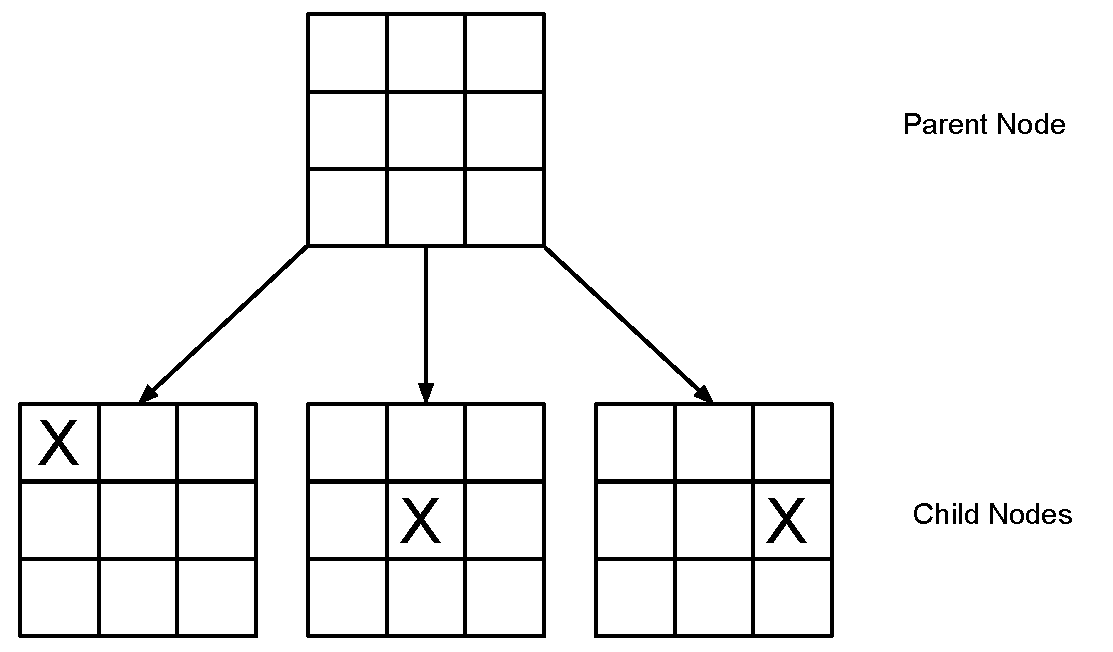
\includegraphics[width=8cm]{TicTacToeTree.pdf}
\centering
\caption{A small portion of what a tree for TicTacToe represents}
\label{fig:TicTacToe}
\end{figure}

Figure \ref{fig:TicTacToe} represents the top portion of a tree for the game TicTacToe. The AI is making the first move, so the root node is the first game board. Each child node represents the potential moves that can be made from the current game state. It is important to note that this figure is a simplification, and that it only shows three of the nine child nodes. Once MCTS decides which move to make, the chosen child node becomes the new root node. For example, if MCTS chose the left child in figure \ref{fig:TicTacToe}, then that child becomes the new root node and its siblings would be discarded.

Along with the game state, each node has an associated value that comes from the simulations performed within that subtree. Only one simulation is performed at each node. Therefore, a subtree of three would have the values from three simulations. With this, we can think of each node as the root of a subtree. The value of that node is representative of the estimated strategic value of the subtree. By choosing the node with the greatest estimated value, the MCTS algorithm is choosing the path with the most number of simulated wins. This means that the MCTS algorithm is maximizing the number of winning moves it can select. This is what MCTS relies on to be effective.   

\subsection{The Four Steps of MCTS}
The process of MCTS is split up into four steps: \textit{selection}, \textit{expansion}, \textit{simulation}, and \textit{backpropagation}. These four steps are iteratively applied until a decision from the AI must be made. Typically, there is a set amount of time that the AI has to make its move, so that is when the algorithm will make its decision.

\begin{figure}[h]
	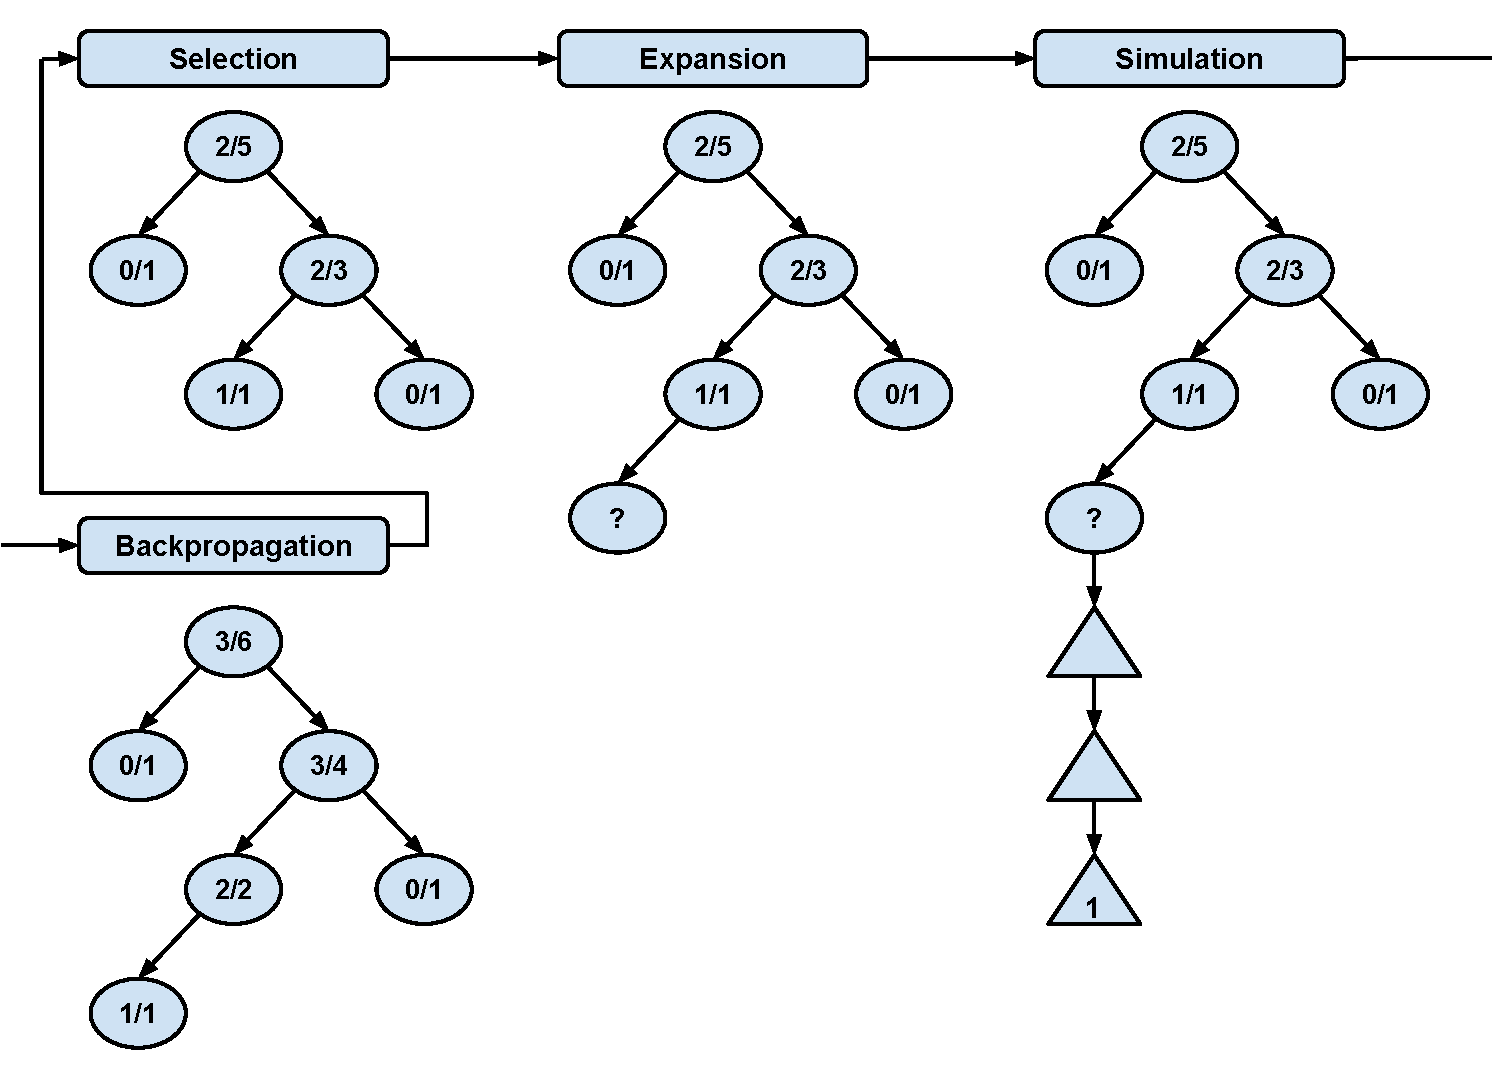
\includegraphics[width=8.5cm]{MCTSFourStepProcess.pdf}
	\centering
	\caption{The four steps of MCTS}
	\label{fig:FourSteps}
\end{figure}

Figure \ref{fig:FourSteps} shows one iteration of the MCTS algorithm with a game tree that only has two legal moves at each node. The first number in each node represents the number of wins in that subtree. The second number is the total number of simulations performed in that subtree. The ratio of these two numbers provides us with the estimated value of each node.

\textbf{Selection} - In the selection process, the MCTS algorithm traverses the current tree using a tree policy. A tree policy uses an evaluation function that prioritize nodes with the greatest estimated value. Once a node is reached in the traversal that has children (or moves) left to be added, then MCTS transitions into the expansion step. In figure \ref{fig:FourSteps}, starting from the root node, the tree policy must make a decision between the 0/1 node and the 2/3 node. Since 2/3 is greater than 0/1, the tree policy will choose the 2/3 node in its traversal. Once at the 2/3 node, the tree policy will then choose the 1/1 node because it is greater than 0/1. This is the first node with children yet to be added, so now MCTS will transition into the expansion step.

\textbf{Expansion} - In the expansion step, a new node is added to the tree as a child of the node reached in the selection step. The algorithm is currently at the 1/1 node, so there is a child node added onto that node indicated by the node with the ?. There is only one node added to the tree in each iteration, and it is at this step.

\textbf{Simulation} - In this step, a simulation (also referred to as a playout or rollout) is performed by choosing moves until either an end state or a predefined threshold is reached. In the case of Go or TicTacToe, an end state is reached when the game ends. Then based on the result of the simulation, the value of the newly added node is established. For example, a simulation for a node in Go reaches the end of a game (the end state), and then determines a value based on whether the player won or lost. In figure \ref{fig:FourSteps} the simulation ended in a 1. Therefore, the value of the new node is 1/1. One simulation resulted in a win, and one simulation has been performed.

In the simulation process, moves are played out according to the simulation policy~\cite{ActionSelection}. This policy may be either weak or strong. A weak policy uses little to no predetermined strategy. It chooses moves randomly from either a subset of the legal moves or from all of the legal moves. A policy may prefer a certain subsection of moves because those moves might be more favorable. Perhaps in the game of TicTacToe the corners are considered to be more favorable. We incorporate this into a simulation policy by having the algorithm randomly choose corner moves until there are no more corner moves left. Then the policy will choose moves at random from the rest of the legal moves. A strong policy uses a more guided approach to choosing moves. A strong policy may make the simulation too deterministic or make it more prone to error~\cite{TheGrandChallenge}, so a weak policy is generally preferred. 

\textbf{Backpropagation} - Now that the value of the newly added node has been determined, the rest of the tree must be updated. Starting at the new node, the algorithm traverses back to the root node. During the traversal the number of simulations stored in each node is incremented, and if the new node's simulation resulted in a win then the number of wins is also incremented. In figure \ref{fig:FourSteps} only the nodes with values 0/1 are not updated since they are not an ancestor of the newly added node. This step ensures that the values of each node accurately reflect simulations performed in the subtrees that they represent.

\subsection{Upper Confidence Bound}

The upper confidence bound applied to trees (UCT) is used by MCTS as the tree policy in the selection step to traverse the tree. UCT balances the idea of exploration versus exploitation. The exploration approach promotes exploring unexplored areas of the tree. This means that exploration will expand the tree's breadth more than its depth. While this approach is useful to ensure that MCTS is not overlooking any potentially better paths, it can become very inefficient very quickly in games with a large number of moves. To help avoid that, it is balanced out with the exploitation approach. Exploitation tends to stick to one path that has the greatest estimated value. This approach is greedy and will extend the tree's depth more than its breadth. UCT balances exploration and exploitation by giving relatively unexplored nodes an exploration bonus.  

 \begin{equation*}
 \label{UCTequation}
 UCT(node) = \frac{W(node)}{N(node)} + \sqrt[C]{\frac{ln(N(parentNode))}{N(node)}}
 \end{equation*}

When traversing the tree, the child node that returns the greatest value from equation \ref{UCTequation} will be selected~\cite{ActionSelection}. N represents the total number of simulations performed at that node and its descendants. W represents how many of those simulations resulted in a winning state. C represents an exploration constant that is found experimentally. The first part of the UCT takes into consideration the estimated value of the node from the ratio of simulations won to total simulations. This is the exploitation part of the equation. The second part of the UCT is the exploration bonus. This compares the total number of simulations performed at the parent node and its descendants to the total number of simulations performed at the examined node and its descendants. This means that the lower the number of simulations that have been performed at this node, the greater this part of the equation will be. 

\section{Using MCTS to play Go}

MCTS has been very successful in its applications in Go. The computer Go programs MoGo and Crazy Stone both use a variation of MCTS, and they have had the best performance of any computer Go programs~\cite{RAVEinGo}. Those programs' variation of MCTS take advantage of certain aspects of Go.

\subsection{All Moves as First (AMAF)}
\textit{All moves as first} (AMAF) is a methodology that treats all moves as if they were the next move played. AMAF does not grant any move extra strategic value based on when it is played. Therefore, in AMAF moves have no contextual dependencies on other moves. This is particularly useful when a move played elsewhere on the board has little or no impact on the move being examined, or if a game arrives at the same state regardless of the order in which the moves are played. 

\begin{figure}[h]
	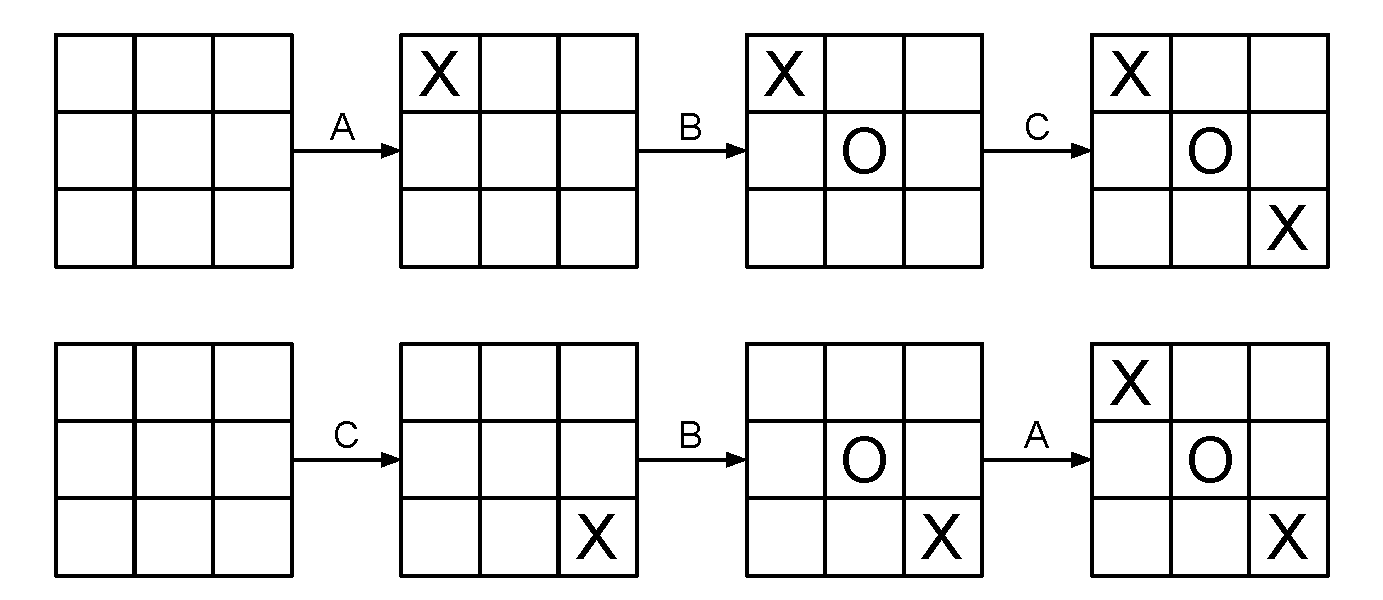
\includegraphics[width=8cm]{MoveOrderNotMattering.pdf}
	\centering
	\caption{Comparison of two sequences of moves in TicTacToe}
	\label{fig:TwoSeq}
\end{figure}

In figure \ref{fig:TwoSeq} are two possible sequences of moves that can be played out in the game TicTacToe. Even though the order of moves A and C are different, it still results in the same game state. AMAF is useful in analyzing the effectiveness of this situation since the order in which the moves are played has no effect strategically. Thus, we can treat playing move A first or move C first as having the same strategic value.

The AMAF methodology is applicable to Go because many of the situations only affect what is happening locally. If a move is made elsewhere on the board, it does not have much of an effect on the strategic value of the move being examined. It is also important to note that in Go a move that repeats a board state is illegal. Therefore, this methodology will not have any inconsistencies with replaying the same move.

\subsection{Rapid Action Value Estimate}
Rapid action value estimate(RAVE) takes the concept of AMAF and applies it to a tree structure. RAVE can be thought of as assigning values to the edges of the tree which represent moves. The value of these moves come from any simulation performed within the subtree in which that move was played. The value is a ratio of these simulations that resulted in a win to the total number of simulations. This is different from MCTS in that MCTS chooses nodes for the strategic value of the game state represented by that node. RAVE chooses nodes for the strategic value of the move.

\begin{figure}[h]
	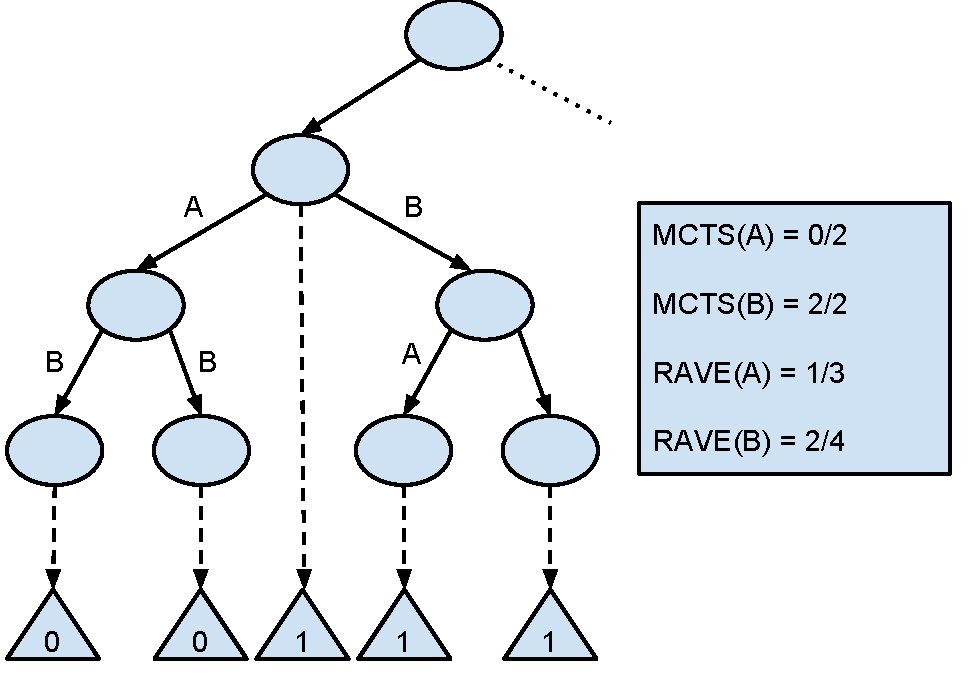
\includegraphics[width=8cm]{RAVEDiagram.pdf}
	\centering
	\caption{MCTS vs RAVE}
	\label{fig:RAVEDiagram}
\end{figure}

Figure \ref{fig:RAVEDiagram} is a comparison between moves A and B from node Z. The dotted lines represent simulations performed at each node with the triangles being the result. In MCTS, the value of A is the value of the node A points to. In this case, A has the value 1/3. Likewise, B has the value 2/3. These values come from the three simulations performed in their respective subtrees. In the RAVE approach, the value for move A is determined by any simulation performed by the descendants of node Z in which A was played. This accounts for the simulation performed in the subtree of B that used move A. Now in RAVE, the value of A is 2/4. The same is true for the RAVE value of B. B was performed in two other simulations in Z's subtree. This makes the RAVE value of B 2/5.

When determining which node to traverse to from node Z, MCTS and RAVE would produce different results. MCTS would choose the node that B is pointing to because the MCTS value of B is greater than the MCTS value of A. RAVE would choose the node A is pointing to because the RAVE value of A is greater than the RAVE value of B.   

The RAVE approach is very powerful and allows us to retrieve much more information out of every simulation. MCTS only gains one piece of information from each simulation. That information is only the result of the simulation. In RAVE, every move performed in a simulation provides us with information. The strategic value of a move in RAVE is developed much more quickly as a result. This means that trees generated by RAVE converge more quickly than trees generated by MCTS.

\subsection{MC RAVE}
The RAVE approach is very useful and efficient, but it can sometimes select an incorrect move~\cite{RAVEinGo}. In Go, when the players have close tactical battles, the sequencing of the moves become very important. In this situation, we cannot treat the moves as AMAF. We still need the contextual dependencies of the MCTS approach.

MC RAVE combines the naive MCTS algorithm and the RAVE approach into one algorithm. MC RAVE stores the values of each node from MCTS and the value of each move from RAVE in the tree structure. MC RAVE takes a weighted average of the two values to determine which node to choose in traversal~\cite{RAVEinGo}. When few simulations have been performed, the RAVE values are given more weight. In this case, RAVE is more accurate because the contextual dependencies of moves are less clear. When a lot of simulations have been performed, the MCTS values will be weighted more heavily. The MCTS values are given more weight because the contextual dependencies of the moves are more strongly developed and are more accurate overall.
\subsection{Go Results}
AI that use more traditional approaches have had very little success playing Go. The deterministic approaches struggle to defeat even low rank amateurs. Now with new Go programs like MoGo and Crazy Stone implementing MC RAVE, AI can compete with top professionals in 9x9 Go~\cite{RAVEinGo}. Not only that, but those programs can even compete against the top pros in handicap games of 19x19 Go. Handicap games let one player start with some number of pieces on the board. That is an incredible feat taking into consideration the immense complexity of a 19x19 board.

\section{Using MCTS for Narrative Generation}
Automated narrative generation is an interesting problem with many applications. One such application is to video games. Narrative generation provides the user with a unique experience on each playthrough which can extend the amount of enjoyment a user receives from a single game. Narrative generation can also be applied as a learning tool. Generating an endless number of fun and interesting stories provides plenty of material for reading practice. These are only two examples, but there are many more ~\cite{Narrative}.

Kartal et al~\cite{Narrative} decided to apply MCTS to narrative generation because of its huge search spaces. Given the success in Go, it makes sense to apply MCTS to narrative generation.

\subsection{Description of Narratives}
The researchers' algorithm uses various predefined actors (or characters), items, locations, and actions to generate a narrative. Actions are used to have actors, items, and locations interact with one another. Here are a few possible actions:
\begin{itemize}
\item \textbf{Move(A, P):} A moves to place P.
\item \textbf{Kill(A, B):} B's health to zero(dead).
\item \textbf{Earthquake(P):} An earthquake strikes at place P. This causes people at P to die (health=0), items to be stuck, and place P to collapse.
\end{itemize}
Each action acts as a function with a list of parameters and a description of what it does. For example, the action \textit{Move} takes a character A and moves them to place P. Actions are important because they are what progress the story. 

In the researchers' algorithm, the user does not provide any of the actions used by the algorithm. However, the user defines the initial setup and goals for the narrative. An initial setup indicates where actors or items are located. For instance, the inspector is in his office, or the lamp is at Becky's house. The narrative goals are what the user wishes to occur in the story. Perhaps the user would like there to be at least two murders and for the murderer to be captured. Given this information, the algorithm will attempt to generate a believable narrative while satisfying the goals set by the user.

\subsection{Tree Representation}
As stated in section \ref{sec:TreeStructure}, the nodes of the MCTS tree represent the entire state at that node. In narrative generation, it is somewhat different. Each node only represents a specific step (or action) of the story instead of capturing the entirety of the narrative up to that point. In order to retrieve the narrative up to a node, we would need to traverse up the tree all the way to the root node. This structuring is similar to the MCTS tree for Go in that to know the sequence of moves leading up to a node, we would need to traverse back to the root. A node by itself does not provide us with the order in which moves are played, only the current state of the game.

In addition to encoding for an action, each node also keeps track of various attributes. Attributes are characteristics of an actor that help maintain the current state of the story. An attribute of an actor might be that actors current health. The health of an actor may go down if attacked. Another example of an attribute is the location of an actor. It would not make much sense if an actor traveled to a location that they are already at which would be possible if the location of the character is not stored.

The researchers' method for tree generation uses a set threshold during the simulation step. The simulation ends when either the narrative has reached a certain length, or when the narrative accomplishes a sufficient percentage of goals. This differs from Go and other games because narratives do not have clear end states. This also means that narrative generation needs a different method of evaluation because the simulations do not simply end in a win or a loss. To address this, the researchers' implemented their own evaluation function, and its details are outlined in section \ref{sec:EvalFunction}. 

\subsection{Evaluation Function}\label{sec:EvalFunction}
The researchers decided they needed a function which considers both believability and goal completion in its evaluation of a narrative~\cite{Narrative}. These two measures are essential for making a quality narrative. A narrative could easily complete the goals defined by the user without being very believable, and a narrative could be very believable while not accomplishing any goals. Sometimes this results in one being sacrificed for the other. Maybe a long series of somewhat unbelievable actions are used for the sake of completing the goals of the narrative. While this outcome is not perfect, it is preferable over the two extremes.

The believability of a narrative is determined by the product of the believability of all of the actions performed throughout the narrative. The believability of a certain action is determined based on its context within the current state of the narrative. This means that certain actions are more or less believable based on previous events or attributes. Character A killing character B is less believable if character A is not angry at character B. Character A looking for clues at character B's house is more believable given that character A is a detective. Each action has its own defined scale of believability ranging from 0 to 1~\cite{Narrative}. The exact details of the scale are outside the scope of this paper, but they can be referenced in the authors' paper~\cite{Narrative}.

Believability is not the only important metric for narrative generation. It is also important that a story completes most, if not all, of the goals defined by the user. The researchers addressed this by determining the percentage of the goals the narrative completes and taking its product with the narrative's believability. Now, the evaluation function considers both the believability and goal completion of a story. 

\subsection{Search Heuristics}
The researchers implemented two different search heuristics into their MCTS algorithm. One heuristic uses selection biasing during the traversal of the tree, and the other uses a rollout biasing while performing simulations.

The selection biasing approach uses a table to store the average value of a specific action. During the traversal of the tree, the algorithm uses the values from the table in combination with the value of a node to determine which node to choose next. The traversal uses a weighted average between the two values. The value from the table is weighted more heavily with fewer simulations, and the value of the node is weighted more heavily with more simulations. This approach is much like the RAVE approach used in Go, but the values are stored in a table instead of in the tree. As such the value from the table is the average value of that action anytime it has been used in any part of the tree. This is different from the RAVE approach in that,
a moves value is only from within a subtree.

The other heuristic the researchers implemented is rollout biasing. This biasing is applied during the simulation step in MCTS. The rollout biasing uses a table, just like the selection biasing, to keep track of the average value of an action. This value is used to bias the random selection of actions in a simulation. If the average value of an action in the table is fairly high, then it is more likely for that action to be chosen. Likewise, if the average value of an action from the table is fairly low, then the action is less likely to be chosen. It is important to make clear that the process is still random, so there will still be variety in the generated narratives.

\subsection{Tree Pruning}
In a game situation, MCTS does tree pruning when a new move is chosen. The siblings that are not chosen are trimmed because they are less promising. Tree pruning allows the algorithm to reallocate the memory used by the less promising nodes for future nodes in the more promising path. The authors needed to incorporate some method of tree pruning into narrative generation because trees generated by MCTS can get very memory intensive.

The authors only allow their MCTS algorithm to plan out the narrative one step at a time. When selecting for the next step, the algorithm runs for a predefined number of iterations. After those iterations are performed, the algorithm chooses the node with the greatest potential value from the child nodes of the previously chosen action. The chosen node effectively becomes the new root node of the tree while keeping the nodes that precede it. When the new node is chosen, all siblings of that node along with their subtrees are discarded.

The authors do note that this approach makes the algorithm no longer probabilistically complete. This means that it is possible that one of the pruned branches is preferable to the current path. Even with this flaw, the authors still found their algorithm to perform reasonably well~\cite{Narrative}.

\subsection{Narrative Generation Results}
The authors compared their implementation of the MCTS algorithm to three different deterministic tree search algorithms: breadth-first search, depth-first search, and best-first search~\cite{Narrative}. Breadth-first search expands each level of the tree before moving on to the next level. Depth-first search expands a tree until an end point is reached. At that point, it backtracks until it finds a new path to expand. Best-first search is a greedy algorithm that expands the tree by choosing nodes with the highest estimated value. Each of these algorithms should provide the optimal solution if given enough time and memory. Depth-first search and Best-first search in particular can find the best solution very early on.

These four algorithms were compared given a low budget of 100 thousand nodes and a high budget of three million nodes. The user goals for this narrative are: at least two actors are killed and the murderer is arrested. Each algorithm was run three times and the score of the resulting narratives were averaged. Here is a table comparing the results: 

\begin{table}[h]
\centering
	\begin{tabular}{ c | c | c | c | c |}
	\cline{2-5}	 
	 & MCTS & Breadth-first & Depth-first & Best-first \\ \hline
	\multicolumn{1}{|p{1.05cm}|}{Low Budget} & 0.07 & 0.05 & <0.001 & 0.005 \\ \hline
	\multicolumn{1}{|p{1.05cm}|}{High Budget} & 0.9 & 0.06 & <0.01 & <0.01 \\ \hline
	\end{tabular}
	\caption[Table caption text]{average scores of the narratives from the different algorithms}
\end{table}

MCTS outperformed the deterministic algorithms with a low budget, and the performance difference is even clearer with the high budget. The authors found that depth-first search failed to meet either of the goals~\cite{Narrative}. Best-first search would use only the most believable actions to accomplish the goals, but used up its allocated memory in trying to do so. Breadth-first search performed the best of the three deterministic algorithms, but its narratives were not very believable.

\begin{figure}[h]
\begin{tabular}{|p{8cm}|}
\hline
Alice picked up a vase from her house. Bob picked up a rifle from his house. Bob went to Alice's house. While there, greed got the better of him and Bob stole Alice's vase! This made Alice furious. Alice pilfered Bob's vase! This made Bob furious. Bob slayed Alice with a rifle! Bob fled to downtown. Bob executed Inspector Lestrade with a rifle! Charlie took a baseball bat from Bob's house. Sherlock went to Alice's house. Sherlock searched Alice's house and found a clue about the recent crime. Bob fled to Alice's house. Sherlock wrestled the rifle from Bob! This made Bob furious. Sherlock performed a citizen's arrest of Bob with his rifle and took Bob to jail. \\ \hline
\end{tabular}
\centering
\caption{high scoring story from MCTS}
\label{fig:GoodStory}
\end{figure}

Figure \ref{fig:GoodStory} is one of the narratives produced by MCTS. It has traits of a quality narrative. It accomplishes both of the goals, and the actions are mostly believable. Bob was aggravated by his interactions with Alice making his actions more believable. There are some problems with the narrative though. It mentions a character named Charlie in one line of the story, and he is never mentioned before or afterwards. Overall, this narrative is reasonable.

\begin{figure}[h]
\begin{tabular}{|p{8cm}|}
\hline
Sherlock moved to Alice's House. An Earthquake occurred at Alice's House! Sherlock and Alice both died due to the earthquake. \\ \hline
\end{tabular}
\centering
\caption{low scoring story from bread-first Search}
\label{fig:BadStory}
\end{figure}

Figure \ref{fig:BadStory} is one of the narratives produced by breadth-first search. While it does accomplish the goal of killing at least two characters, it fails to accomplish the more complex goal of arresting the murderer. This narrative is not very believable. Worse, it is not very interesting. Hardly anything happens in it. It ends after only three lines. It is clear which algorithm performed better just from reading the resulting narratives regardless of their scores. 

\section{Conclusions}
The Monte Carlo tree search algorithm has been very successful in extending the capabilities of AI. MCTS performs reasonably well on problems with vast search spaces, which were very difficult for previous algorithms. Before MCTS, AI struggled to defeat low rank amateurs in Go. Now with MCTS, AI can compete with high level pros~\cite{TheGrandChallenge}. Also, MCTS has demonstrated its effectiveness in generating narratives, another problem with vast search spaces~\cite{Narrative}.

MCTS has applications outside of problems with larger search spaces. MCTS can outperform humans in many puzzles and real time games~\cite{Narrative}. MCTS can compete with other top algorithms in playing the video game Super Mario Brothers~\cite{Jacobsen:2014}. Between its success in vast search spaces and the variety of its applications, MCTS will certainly continue to be a prominent algorithm in the field of artificial intelligence.

\section{Acknowledgements}

% The following two commands are all you need in the
% initial runs of your .tex file to
% produce the bibliography for the citations in your paper.
\bibliographystyle{abbrv}
% sample_paper.bib is the name of the BibTex file containing the
% bibliography entries. Note that you *don't* include the .bib ending here.
\bibliography{MaxMagnusonSeniorSeminarPaper}  
% You must have a proper ".bib" file
%  and remember to run:
% latex bibtex latex latex
% to resolve all references

\end{document}
